\chapter{Introduction and Physics Background}
\section{Units and Conventions}
\label{sec:units_and_conventions}
    Even though nature does not establish preferred units, the physics that describes it requires establishing a common language and framework.
    %
    In high energy physics, the choice of units reflects a not simply an arbitrary choice, but a philosophical stance about the nature of reality.
    %
    While everyday experience suggests that meters, kilograms, and seconds might be the most suitable units to express the physical world, particle physics reveals that speed, action, and energy form more natural rulers for measuring the universe at its smallest scales.
    %
    \begin{definition}
        \emph{Natural Units} are a system where \(\hbar = c = 1\), effectively setting the speed of light and quantum of action as fundamental measuring sticks.
        %
        This choice transforms all physical quantities into powers of energy.
    \end{definition}
    
\begin{table}
    \centering
    \caption[Unit conversions in natural units]{%
      Combined unit conversions in natural units, showing both abbreviated and full natural unit expressions, their SI equivalents and their physical significance.
    }
    \label{tab:unit-conversions-combined}
    \begin{tabular}{@{} l c c l p{5cm} @{}}
      \toprule
      Quantity           & Abbrev.               & Full Natural Units                & SI Conversion                                                    & Comment                                           \\
      \midrule
      Speed              & \(c\)                 & \(1\,c\)                          & \(3\times10^{8}\,\mathrm{m/s}\)                                   & Speed of light                                    \\
      Angular Momentum   & \(\hbar\)             & \(\hbar\)                         & \(1\times10^{-34}\,\mathrm{m^{2}\,kg/s}\)                         & Quantum of action                                 \\
      Energy             & \(\mathrm{GeV}\)      & \(\mathrm{GeV}\)                  & \(1\,\mathrm{GeV}=1.602\times10^{-10}\,\mathrm{J}\)               & Natural nuclear‐binding scale                     \\
      Momentum           & \(\mathrm{GeV}\)      & \(\mathrm{GeV}/c\)                & \(1\,\mathrm{GeV}/c=5.344\times10^{-19}\,\mathrm{kg\,m/s}\)       & Typical LHC particle momentum                     \\
      Mass               & \(\mathrm{GeV}\)      & \(\mathrm{GeV}/c^{2}\)            & \(1\,\mathrm{GeV}/c^{2}=1.783\times10^{-27}\,\mathrm{kg}\)        & Proton mass \(\approx0.938\,\mathrm{GeV}\)        \\
      Length             & \(\mathrm{GeV}^{-1}\) & \(\hbar c/\mathrm{GeV}\)          & \(1\,\mathrm{GeV}^{-1}=1.973\times10^{-16}\,\mathrm{m}\)           & Compton wavelength scale                          \\
      Time               & \(\mathrm{GeV}^{-1}\) & \(\hbar/\mathrm{GeV}\)            & \(1\,\mathrm{GeV}^{-1}=6.582\times10^{-25}\,\mathrm{s}\)           & Natural oscillation period                       \\
      Charge             & \(e/\sqrt{4\pi\alpha}\)& \(e/\sqrt{4\pi\alpha}\)          & \(5.3\times10^{-19}\,\mathrm{C}\)                                 & Elementary charge \(e=1.6\times10^{-19}\,\mathrm{C}\) \\
      Cross Section      & \(\mathrm{GeV}^{-2}\) & \(\mathrm{GeV}^{-2}\)             & \(1\,\mathrm{GeV}^{-2}=3.894\times10^{-32}\,\mathrm{m^{2}}\)      & \(1\text{ barn}=2.568\times10^{-9}\,\mathrm{GeV}^{-2}\) \\
      Magnetic Field     & \(\mathrm{GeV}^{2}\)  & \(\mathrm{GeV}^{2}/(\hbar c^{2})\)& \(5\times10^{16}\,\mathrm{T}\)                                    & Typical magnetic‐field scale                      \\
      \bottomrule
    \end{tabular}
  \end{table}
The beauty of natural units emerges when considering quantum field theory. The Klein-Gordon equation for a scalar field φ:
(∂²/∂t² - ∇² + m²)φ = 0
reveals that mass m has dimensions of inverse length - it sets the characteristic scale over which quantum fields oscillate. A particle with mass 1 GeV has a Compton wavelength of approximately 0.2 femtometers, roughly the size of a proton.
Coordinate Systems and Relativistic Geometry
At a hadron collider, the choice of coordinates must respect the underlying symmetries of the physics. The laboratory frame provides a natural Cartesian system:

z-axis: Along the beam direction (longitudinal)
x-axis: Horizontal, pointing toward the center of the accelerator ring
y-axis: Vertical, completing the right-handed system

However, the partons within colliding hadrons carry unknown fractions of the beam momentum, making the center-of-mass frame of each collision unknowable. This fundamental uncertainty motivates a coordinate system that transforms simply under longitudinal Lorentz boosts.

Pseudorapidity (η): Defined as η = -ln[tan(θ/2)], where θ is the polar angle from the beam axis. Under a longitudinal boost with velocity β, a massless particle's η transforms as η → η + tanh⁻¹(β).

The mathematical elegance of pseudorapidity becomes apparent when we expand its definition:
η = -ln[tan(θ/2)] = (1/2)ln[(|p| + pz)/(|p| - pz)] = tanh⁻¹(pz/|p|)
For massless particles, differences in η remain invariant under longitudinal boosts, motivating the ubiquitous angular distance metric:
ΔR² = Δη² + Δφ²
where φ is the azimuthal angle around the beam axis. This metric approximates the geometric angle between particles in the detector while remaining approximately boost-invariant.

\section{The Standard Model: Theoretical framework}
The Standard Model of particle physics represents one of the most significant intellectual achievements in modern science.
%
Developed throughout the latter half of the $20^{th}$ century, it provides a quantum field theory framework that describes three of the four known fundamental forces—the electromagnetic, weak, and strong interactions---along with classifying all known elementary particles.
%
The mathematical formulation of the Standard Model is based on gauge theory, specifically quantum chromodynamics (QCD) and the electroweak theory, underpinned by the gauge symmetry group \(SU(3)\times SU(2)\times U(1)\).

The predictive power of the Standard Model has been repeatedly validated through precision experiments across multiple energy scales, from low-energy nuclear phenomena to the highest energy particle collisions achievable at modern accelerators.
%
Its crowning achievement came with the discovery of the Higgs boson in 2012 at the Large Hadron Collider (LHC)~\cite{ATLAS:2012yve, collaboration_observation_2012}, confirming the mechanism through which elementary particles acquire mass.
%
A schematic illustration of the standard model can be found in \cref{fig:sm}.

\begin{figure}
    \centering
    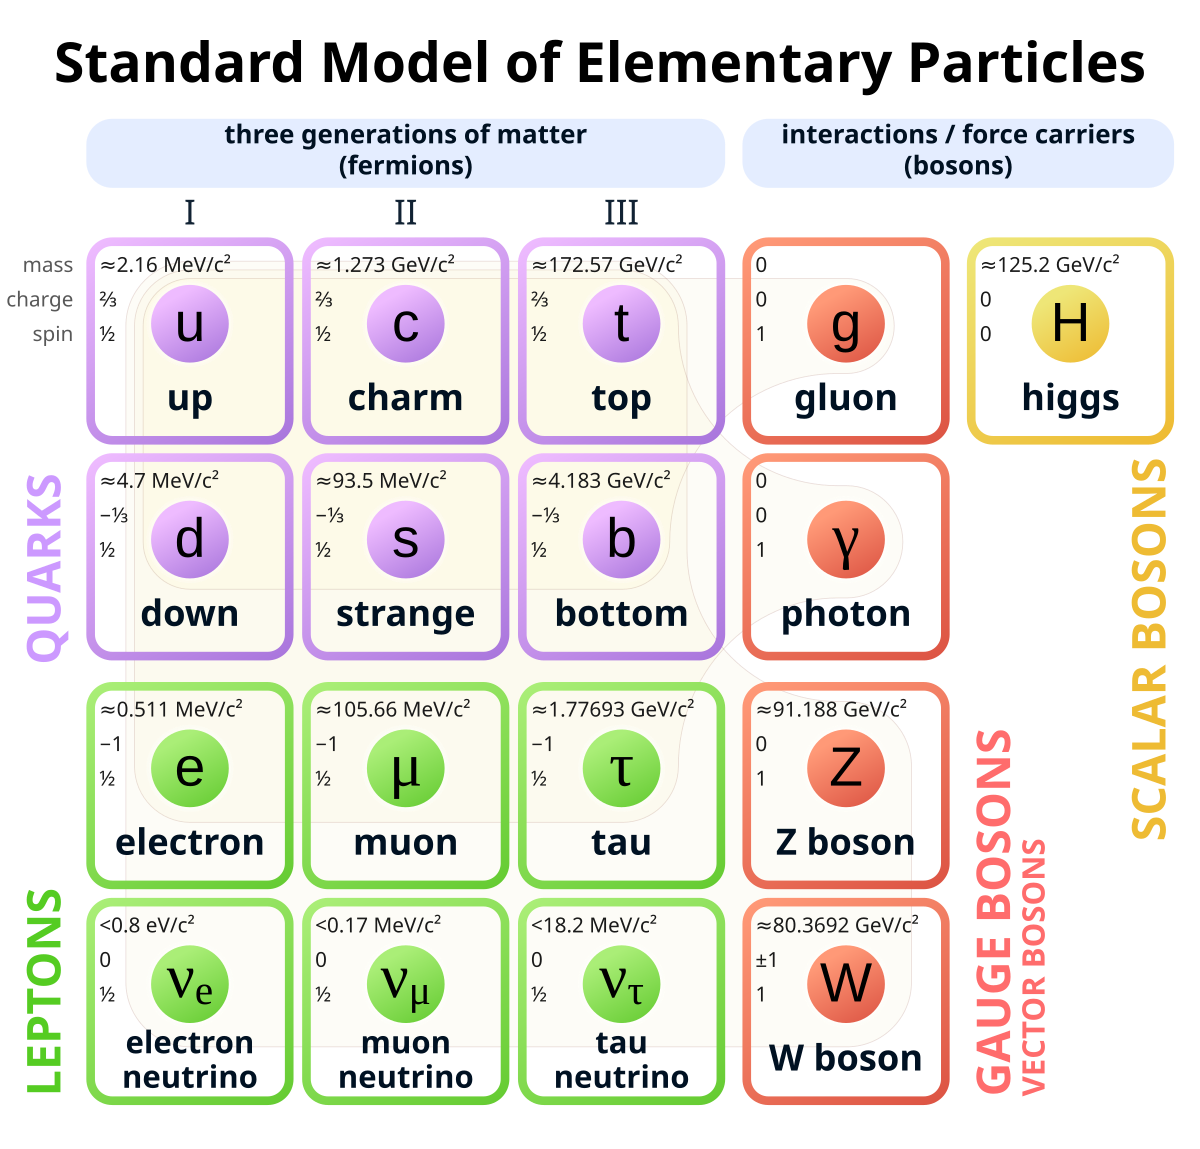
\includegraphics[width=0.5\linewidth]{figures/chapter-01/Standard_Model_of_Elementary_Particles.svg.png}
    \caption{
        A schematic illustration of the Standard Model~\cite{wiki:stdmodel}.
    }
    \label{fig:sm}
\end{figure}
\subsection{Fundamental Particles and Forces}
The Standard Model categorizes elementary particles into two main families: fermions, which comprise matter, and bosons, which mediate forces between matter particles.
\subsubsection{Fermions: The Building Blocks of Matter}
Fermions, characterized by half-integer spin, obey the Pauli exclusion principle and are further classified into quarks and leptons, each arranged in three generations of increasing mass:
\paragraph{Quarks} (spin $ = \nicefrac{1}{2}$)
Quarks are catagorized into three generations as follows:
\begin{itemize}
    \item Up (u) and down (d),
    \item Charm (c) and strange (s),
    \item Top (t) and bottom (b).
\end{itemize}

Quarks carry fractional electric charge and color charge, and experience all fundamental forces.
%
They are confined within hadrons---composite particles categorized as baryons (three--quark states, like protons and neutrons) or mesons (quark--antiquark pairs).

\paragraph{Leptons} (spin $ = \nicefrac{1}{2}$)
Like quarks, leptons too are catagorized into three generations.
\begin{itemize}
    \item Electron (e) and electron neutrino ($\nu_e$),
    \item Muon $(\mu)$ and muon neutrino ($\nu_\mu$),
    \item Tau ($\tau$) and tau neutrino ($\nu_\tau$).
\end{itemize}

Electrons, muons, and taus carry unit electric charge and interact via electromagnetic and weak forces, while neutrinos are electrically neutral and interact only through the weak force, making them notoriously difficult to detect.

\subsubsection{Bosons: Force Carriers}
Bosons, with integer spin values, mediate the fundamental interactions. The Standard Model comprises the following bosons:
\begin{itemize}
    \item Photon $(\gamma)$: The massless spin--1 boson mediating the electromagnetic force,
    \item $W^\pm$ and $Z$ bosons: Massive spin--1 bosons mediating the weak force
    \item Gluons $(g)$: Eight massless spin--1 bosons mediating the strong force
    \item Higgs boson ($H$): A massive spin--0 boson associated with the Higgs field that gives mass to elementary particles
\end{itemize}

\subsection{Theoretical Framework and Symmetries}
The Standard Model is constructed through principles of quantum field theory where particles are excitations of underlying quantum fields.
%
Its mathematical structure is determined by local gauge invariance under the following specific symmetry transformations
\begin{itemize}
    \item $U(1)_Y$: Associated with weak hypercharge, the symmetry of electroweak theory
    \item $SU(2)_L$: Describes the weak isospin, acting on left-handed fermions
    \item $SU(3)_C$: Governs the strong interactions through color charge in QCD
\end{itemize}

Electroweak unification, demonstrated by Glashow~\cite{Glashow:1961tr}, Weinberg~\cite{Weinberg:1979pi}, and Salam~\cite{Salam:1980jd}, demonstrates how the electromagnetic and weak forces emerge as different aspects of a single electroweak interaction, which undergoes spontaneous symmetry breaking at low energies.

\subsection{The Higgs Mechanism and Mass Generation}
The Higgs mechanism, proposed by several physicists including Peter Higgs in the 1960s~\cite{PhysRevLett.13.508}, addresses the theoretical inconsistency of massive gauge bosons in a gauge-invariant theory.
%
The mechanism introduces a scalar field---the Higgs field---that permeates space and spontaneously breaks the electroweak symmetry when the universe cooled after the Big Bang.
%
This symmetry breaking generates masses for the W and Z bosons while leaving the photon massless, explaining the significant difference between the electromagnetic and weak forces at ordinary energies. Additionally, the Higgs field couples to fermions through Yukawa interactions~\cite{DHoker1984DecouplingTheory}, generating their masses with coupling strengths proportional to the particle masses.

The discovery of the Higgs boson at the LHC in 2012, with properties consistent with Standard Model predictions, provided crucial experimental validation of this mechanism and completed the Standard Model's particle roster.

\subsection{Limitations and Beyond the Standard Model (BSM) Physics}
Despite its remarkable success, the Standard Model has several well-recognized limitations, including

    \begin{itemize}
        \item It does not incorporate gravity, the fourth fundamental force.
        \item It fails to explain the observed matter--antimatter asymmetry in the universe.
        \item It does not account for dark matter or dark energy, which together constitute about 95\% of the universe's energy content.
        \item  It requires fine-tuning of parameters, raising theoretical concerns like the hierarchy problem.
        \item  It does not explain neutrino masses, which must exist given observed neutrino oscillations.
    \end{itemize}
These limitations motivate theoretical extensions and experimental searches for physics beyond the Standard Model, including supersymmetry, grand unified theories, and various dark matter candidates.
%
Precision measurements at particle physics experiments provide one of the most powerful approaches to probe these potential extensions, making analysis techniques like those discussed in this thesis essential for advancing our fundamental understanding of nature.

\section{Fundamental role of cross section measurements in particle physics}

Differential cross section measurements are the fundamental currency of scientific exchange in particle physics, serving as the primary bridge between theoretical predictions and experimental observations.
%
These measurements quantify the probability density of specific particle interactions as a function of kinematic variables, providing the essential link between theoretical predictions and experimental observations.
%
 A cross section quantifies the probability of a specific particle interaction occurring and is typically expressed in units of area (barns, where $1$ barn $= 10^{-24} \mathrm{cm}^2$). This seemingly simple concept forms the cornerstone of how we test and validate our understanding of fundamental physics.
 
The Standard Model of particle physics---our most successful theory describing elementary particles and their interactions---makes precise predictions for cross sections that can be directly tested at particle physics experiments.
%
Any statistically significant deviation between measured cross sections and theoretical predictions may signal the presence of new physics beyond the Standard Model~\cite{particle_data_group_review_2022}.\footnote{Such deviations might also signal errors in the theoretical framework used for predictions or in the experimental procedures used to measure the cross section.
} 

Cross sections are particularly powerful because they encode the underlying quantum field theory structure in a form that can be directly probed by experiment.
%
For instance, measurements of jet production cross sections at different energy scales reveal the running of the strong coupling constant \(\alpha_S\)~\cite{chiefa_parton_2025}, while precision electroweak cross section measurements constrain the properties of the Higgs boson and other fundamental particles~\cite{noauthor_precision_2006}.
%
In searches for physics beyond the Standard Model, differential cross section measurements can reveal subtle deviations that point to new particles or interactions, even when direct observation is beyond experimental reach.

These measurements also serve a crucial role in constraining effective field theories (EFTs) that parameterize potential new physics in a model-independent way.
%
By measuring differential distributions with high precision, experiments can place bounds on EFT coefficients, narrowing the space of viable theoretical extensions to the Standard Model~\cite{contino_validity_2016}.
%
The ongoing precision program at the Large Hadron Collider (LHC) relies heavily on refined cross section measurements to extract maximum physical insight from collected data.
%
In addition to driving comparisons with theoretical models, cross section measurements are also used at high energy physics experiments for MC tuning~\cite{albert_antares_2025} and consistency checks~\cite{buckley_constraints_2025} among other applications.

\section{Cross Section Measurements: From Theory to Experiment}
\subsection{Theory}
    Classically, the cross section (\(\sigma\)) represents the effective area within which two particles must interact for a particular process to occur.
%
For collisions between discrete particles, the cross section is defined as the area transverse to their relative motion.
%
If the particles were to interact via contact forces (e.g., hard spheres), the cross section corresponds to their geometric size.
%
For long--range forces however, (e.g., electromagnetic or gravitational interactions), the cross section is larger than the physical dimensions of the particles due to action-at-a-distance effects.
%
The differential cross section (\(\frac{d\sigma}{d\Omega}\)) provides additional granularity by describing how the probability of scattering depends on specific final-state variables, such as scattering angle (\(\theta\)) or energy transfer. It is defined as
\begin{equation}
    \frac{\dd\sigma}{\dd\Omega} = \frac{\text{Number of events scattered into } \dd\Omega}{\text{Incident flux} \times \text{Target density}}.
\end{equation}

The total cross section can be recovered by integrating over solid angle:
\begin{equation}
\sigma = \int_{4\pi} \frac{\dd\sigma}{\dd\Omega} \, \dd\Omega.
\end{equation}

    While the classical picture above is intuitive, scattering at HEP experiments is governed by quantum field theory (QFT).
    %
    In this framework the probability for a process is encoded in a Lorentz‑-invariant matrix element \(\mathcal{M}\).
    %
    For a \(2 \to n\) reaction with incoming four‑-momenta \(p_{1,2}\) and final‑state phase space \( \text{d}\Phi_n \), the fully differential cross section is

    \begin{equation}
      \dd\sigma =
      \frac{(2\pi)^4 \, \delta^{(4)}\!\bigl(p_1 + p_2 - \sum_{i=1}^n p_i\bigr)}
           {4\,\sqrt{(p_1\!\cdot\!p_2)^2 - m_1^2 m_2^2}}
      \; |\mathcal{M}|^2 \;
      \dd\Phi_n,
      \label{eq:qft_xsec}
    \end{equation}
    where the denominator is the flux factor and \(\dd\Phi_n = \prod_{i=1}^{n} \tfrac{\dd^3 p_i}{(2\pi)^3 2E_i}\) is the Lorentz‑-invariant phase0‑space element.\footnote{Standard derivations can be found in \cite{peskin_introduction_1995,Navas2024ReviewPhysics, Hollik2014Quantum978-1-107-03473-0, QuantumAssessment}.
    }
    %
    \cref{eq:qft_xsec} reduces to the classical area when \(|\mathcal{M}|^2\) is replaced by a contact interaction and the final‑-state integral collapses to a single kinematic configuration.
    %
    Integrating \cref{eq:qft_xsec} over final‑state kinematics yields the total cross section, \(\sigma = \int \dd\sigma\).
    %
    At tree level, \(|\mathcal{M}|^2\) is computed from Feynman rules derived from the Lagrangian, while higher‑-order corrections incorporate loops, parton showers, and non‑-perturbative effects such as hadronisation.
    %
    For practical experimental predictions predictions one folds \(|\mathcal{M}|^2\) with parton distribution functions (PDFs) and convolutes the result with detector response---precisely the forward problem addressed by the unfolding methods developed in this thesis.

Differential cross sections are have a long history of providing valuable insights for probing fundamental properties of particles and interactions.
%
For example, Rutherford scattering experiments revealed the existence of atomic nuclei by analysing angular distributions of scattered alpha particles \cite{F.R.S.1911LXXIX.Atom}.

    \subsection{Experimental Measurement}
    \label{subsec:exp_measurement}
        At modern colliders\footnote{
            This section focusses on collider experiments, but similar analyses can be applied to non--collider HEP experiments as well, such as fixed target experiments.
            %
            \cite{leo_techniques_1994} and \cite{particle_data_group_review_2022} chapters 31--38 provide a comprehensive and detailed exposition of experimental measurement in HEP.
            %
            \cite{Brodsky2013PhysicsBeams, AveryCrossRates} focus specifically on fixed target techniques and phenomenology.
            %
            \cite{MuheimNuclearLaws} compares collider and fixed--target formalisms, reviews luminosity analogues, and details the role of detector simulations and unfolding in a fixed-target context
        } the two beams themselves act as both ``projectile" and ``target." 
        %
        The fundamental experimental quantity is the instantaneous \emph{luminosity} \(\mathcal{L}(t)\), defined such that the interaction rate for a process with cross section \(\sigma\) is \(\dd N/\dd t = \mathcal{L}(t)\,\sigma\).

        Time-‑integrating over a data‑-taking period \([t_0, t_f]\) yields the \emph{integrated luminosity},
        \begin{equation}
          \mathcal{L}_{\text{int}}
          = \int_{t_0}^{t_f} \mathcal{L}(t)\,\dd t,
          \qquad
          \sigma
          = \frac{N_{\text{obs}} - N_{\text{bkg}}}
                 {\mathcal{L}_{\text{int}}\,\epsilon\,A}.
          \label{eq:crossec_collider}
        \end{equation}
        Here \(N_{\text{obs}}\) is the number of selected events, \(N_{\text{bkg}}\) an estimate of background contaminations, \(\epsilon\) the detector and selection efficiency, and \(A\) the geometric‑-plus-‑kinematic acceptance of the analysis.

        For binned measurements one bins events in an observable \(X\) (e.g.\ transverse momentum \(p_T\) or rapidity \(y\)) and divides by the bin width
        \begin{equation}
          \frac{\dd\sigma}{\dd X}\Big|_{X_i}
          = \frac{1}{\mathcal{L}_{\text{int}}\,\Delta X_i}
            \frac{N_i^{\text{obs}} - N_i^{\text{bkg}}}
                 {\epsilon_i\,A_i},
          \label{eq:diff_crossec_collider}
        \end{equation}
        with the index \(i\) denoting the \(i-\)th bin.

        Luminosity determination is itself a precision measurement, usually performed with dedicated luminometers that exploit van‑-der-‑Meer
        scans or pile-‑up counting techniques.
        %
        The efficiency–acceptance term \(\epsilon\,A\) is obtained from full detector simulations and corrected in data using control samples and ``tag-‑and-‑probe" methods.

        Equations~\eqref{eq:crossec_collider}–\eqref{eq:diff_crossec_collider} thus link the theoretically calculated parton‑level cross sections (cf.\ Eq.\;\eqref{eq:qft_xsec}) to the raw observables recorded by the a detector, completing the chain from theory to experiment.

    \subsection{Applications in Particle Physics}
        As mentioned above, cross section measurements serve as the fundamental currency of particle physics, translating abstract theoretical predictions into measurable experimental quantities.
        %
        However, their applications extend far beyond simple theory validation into the operational heart of how experiments function, analyse data, and cross--validate results.
        \subsubsection{Theory validation}
            Comparing measured cross sections with predictions from quantum field theory validates and tests theoretical models like Quantum Chromodynamics (QCD) and electroweak theory, by encapsulating interaction probabilities in a measurable form.
            %
            Deviations from expected cross sections may indicate new phenomena, such as supersymmetric particles or dark matter candidates.
            %
            Differential cross sections also provide constraints on effective field theories and parton distribution functions (PDFs), essential for understanding the internal structure of hadrons.
            %
            Unfolded cross section measurements allow comparisons with theoretical models years after data collection, even if detector simulations are no longer available, further enhancing their utility, and future proofing the data.
            %
            Their determination requires careful experimental design and analysis techniques to account for systematic uncertainties introduced by detector effects.

        \subsubsection{Monte Carlo Tuning}
            Monte Carlo Tuning is the iterative process of adjusting simulation parameters to match measured cross sections, ensuring that detector simulations accurately reproduce real experimental data.
            %
            Many Measurements are extensively used in Monte Carlo (MC) tuning.
            %
            Every particle physics analysis relies on sophisticated simulations that model everything from the initial parton interactions through hadronization to detector response.
            %
            These simulations contain dozens of phenomenological parameters, from the strong coupling constant at various scales to non-perturbative fragmentation functions.
            %
            Measured cross sections provide the ground truth that anchors these simulations to reality.

            Consider the following example:
            %
            When CMS measures the inclusive jet cross section at a new centre-of-mass energy, that measurement immediately becomes a crucial input for tuning generators like \textsc{Pythia} or \textsc{Herwig}.
            %
            The differential distributions---whether in transverse momentum, rapidity, or invariant mass---reveal where our models succeed and where they fail.
            %
            A discrepancy in the high\(-p_T\) tail might indicate we need to adjust our modelling of initial--state radiation; unexpected structure in angular distributions could point to missing higher--order QCD effects.
        \subsubsection{Consistency Checks}
            Cross--validations between different experimental approaches, detector configurations, or analysis methods to ensure measurement reliability and identify systematic biases.
            %
            Cross sections also serve as essential consistency checks across multiple dimensions of experimental physics.
            %
            Within a single experiment, measuring the same process through different decay channels provides a powerful systematic cross--check.
            %
            For instance, measuring the W boson production cross section through both electronic and muonic decays tests our understanding of lepton universality while simultaneously validating detector calibrations.
            %
            Any significant deviation signals either new physics, errors in the phenomenological method used, or unaccounted systematic effects.
            
            Between experiments, cross section measurements enable crucial cross--experiment validation.
            %
            When CMS and ATLAS measure the same process with independent detectors and analysis chains, agreement within uncertainties validates both measurements.
            %
            Disagreement, conversely, triggers investigations that can reveal subtle systematic effects or push calculations to higher precision.

            The applications cascade through every level of experimental operations.
            %
        \subsubsection{Luminosity determination}
            Luminosity determination becomes possible through processes with well--known theoretical cross sections.
            %
            Van der Meer scans calibrate the absolute luminosity scale, but elastic scattering and other standard candle processes provide continuous monitoring.
            %
            The uncertainty on integrated luminosity, typically \(2-3\%\), directly impacts every cross section measurement, creating a web of interdependencies.
            
        \subsubsection{Background estimation}
            Background estimation in searches for new physics relies on measured cross sections of Standard Model processes.
            %
            When searching for supersymmetric particles, the irreducible backgrounds from \(W+\)jets or \(t\bar t\) production must be understood at the percent level.
            %
            Control regions enriched in these backgrounds, combined with precise cross section measurements, enable data--driven background estimates that would be impossible from simulation alone.
        \subsubsection{Parton Luminosity}
            Parton luminosity is effective luminosity for specific parton--parton interactions, calculated by convolving the total luminosity with parton distribution functions.

            A particularly elegant application of cross sections emerges in parton luminosity calculations.
            %
            Since protons are composite objects, the effective luminosity for producing heavy particles depends on the convolution of PDFs with the partonic cross section.
            %
            Measurements of Drell--Yan production at different invariant masses directly probe the quark and antiquark distributions, while inclusive jet production constrains the gluon PDF.
            %
            This creates a self--consistent feedback loop, where better PDFs enable more precise predictions, which enable more sensitive measurements, which further constrain the PDFs.
            
        \subsubsection{Detector Performance Validation}
             Detector performance validation represents another major application of cross section measurements.
             %
             Measured cross sections for well--understood processes serve as standard candles for monitoring detector stability over time.
             %
             For example, slow drift in the measured \(Z\to\mu\mu\) cross section might indicate degrading muon chamber performance long before it would be noticed in individual event displays.
             %
             These measurements become part of the experiment's data quality monitoring, flagging problems in real--time.
            \subsubsection{Systematic uncertainty evaluation}
                The role in systematic uncertainty evaluation cannot be overstated. Every measurement must account for theoretical uncertainties in signal and background processes. By measuring auxiliary cross sections—for instance, Z+jets production when studying W+jets—experiments can constrain these uncertainties using data rather than relying solely on theoretical estimates. This in-situ constraint often reduces systematic uncertainties by factors of two or more.
            \subsubsection{Future planning}
                Finally, cross sections enable physics program planning for future experiments.
                %
                The measured production rates at current energies, extrapolated using theoretical calculations, determine required luminosities and detector capabilities for next--generation experiments.
                %
                For exmaple, the surprisingly large Higgs production cross section at the LHC, for instance, has already influenced design considerations for future electron--positron Higgs factories.
                
    In sum, cross sections certainly do function as the Rosetta Stone of particle physics, translating between the languages of theory, simulation, and experimental measurement while maintaining coherence across all three domains.
    %
    But they serve not merely as endpoints of analyses but as the connective tissue that binds together theory, simulation, and experiment into a coherent whole.
    %
    They simultaneously test our understanding, calibrate our tools, and point the way toward new discoveries.
    %
    This multiplicative utility explains why cross section measurements, even of well--studied processes, remain priorities for every particle physics experiment.

\section{Detector response in precision measurements}
    The direct comparison between theoretical predictions and experimental measurements is complicated by detector effects.
    %
    HEP detectors are technological marvels that capture the trajectories of charged particles, energy deposits in calorimeters, and timing and pattern--recognition information from tracking and particle--identification systems, but they introduce distortions that must be carefully accounted for to extract the true physical distributions of interest.
    %
    Particle physics detectors represent some of humanity's most sophisticated sensing apparatus—--capturing particle trajectories with silicon sensors operating at liquid helium temperatures, measuring energy deposits in dense calorimeter crystals, and reconstructing vertices with sub--millimetre precision.
    %
    Yet these technological marvels inevitably introduce systematic distortions that transform the pristine theoretical predictions into the messy reality of experimental data.
    
    Consider the information degradation that occurs in every measurement. 
    %
    Finite resolution creates fundamental blurring, much like how a camera lens distorts an image.
    %
    The detector's discrete sensing elements can only measure particle energies, momenta, and positions to finite precision, creating an inherent convolution between the true physics distribution and the instrument response function.
    %
    Geometric acceptance imposes hard boundaries on observable phase space.
    %
    Particles scattered into the forward beam pipe or extreme backward angles simply vanish from the recorded dataset, creating holes in the measurement that no amount of statistics can fill.
    
    Detection efficiency varies across the detector's active volume, introducing a complex weighting function that depends on particle type, energy, and trajectory.
    %
    A high--energy muon might traverse the entire detector with near--perfect efficiency, while a low--energy hadron could be absorbed in the first layers of material.
    %
    Particle misidentification compounds these challenges through cross--contamination between categories, such as when hadronic shower fluctuations cause a pion to masquerade as a kaon~\cite{belle_collaboration_precision_2013}.

    In this way every detector measurement embeds two irreducible probability relationships.
    \begin{enumerate}
        \item Detection incompleteness: \(p(\text{measured}|\text{true}) < 1\) True events that fail to be recorded
        \item Measurement impurity: \(p(\text{true}|\text{neasured}) < 1\) Recorded events that represent background contamination
    \end{enumerate}
    This reveals why detector corrections are fundamentally different from simple calibrations.
    %
    Unlike adjusting a scale that consistently reads, say, \(5\%\) high, detector response involves dual information loss that operates asymmetrically.
    %
    The first inequality captures the selection bias where certain true configurations have zero probability of detection, creating null spaces in the measurement.
    %
    The second inequality captures the contamination bias where every reconstruction category contains some fraction of misclassified events.
    
    Background contamination represents a third problem---every measurement category contains some admixture of misclassified events.
    %
    When hadrons interact in electromagnetic calorimeters, they can mimic electron signatures.
    %
    When cosmic ray muons traverse the detector during a collision, they contribute to the muon count despite having no connection to the physics of interest.
    %
    This contamination creates what signal processing engineers call the false positive rate.
    
    The mathematical relationship between true particle level distributions and observed detector level measurements follows the convolution integral
    \[
        \label{eq:forward-folding}
        p(x) = \int r(x|z)\;p(z)\; \dd z
    \]
    Where \(p(x)\) is the detector level density, \(p(z)\) is the particle level density and \(r(x|z)\) serves as the response kernel, the conditional probability density that maps each possible true configuration \(z\) to the distribution of possible detector measurements \(x\).
    %
    This kernel encapsulates the entire cascade of finite resolution information degradation.
    
    The response kernel is analogous to the optical transfer function in image processing.
    %
    It describes how the ``lens" of the detector blurs and distorts the perfect theoretical ``image".
    %
    The response function inherently embeds both probabilistic asymmetries.
    %
    Regions where \(\int r(x|z)\;\dd x < 1\) reveal acceptance holes, i.e. true configurations that produce no detector signal whatsoever.
    %
    Conversely, the convolution structure itself ensures that multiple truth distributions can yield identical detector observations, creating the degeneracy problem that makes direct inversion impossible.
    
    A central challenge then for particle physics is inverting this response kernel to recover \(p(z)\) from observed data \(p(x)\).
    %
    This inversion is mathematically ill--posed precisely because of the information loss.
    %
    Standard matrix inversion fails catastrophically, amplifying statistical noise into wild oscillations that bear no resemblance to the underlying physics.
    
    The resolution requires sophisticated regularization methods that impose additional constraints such as smoothness assumptions, positivity requirements, and prior knowledge about the expected signal shape.
    %
    These constraints transform the ill--posed inverse problem into a well--defined statistical inference challenge, though at the cost of introducing systematic uncertainties that must themselves be carefully validated.
    
    The detector response problem exemplifies a universal pattern in experimental science: the tension between instrumental precision and information preservation.
    %
    From astronomical imaging through medical diagnosis to HEP measurements, the fundamental trade off between sensitivity and purity governs all attempts to extract signal from noise.

\section{Challenges at modern experiments}
Several challenges at the modern HEP experiments make cross section measurements particularly demanding.

    \begin{itemize}
        \item \textbf{High--dimensional phase spaces}: Modern measurements often involve multiple correlated observables, creating high--dimensional distributions that are difficult to analyze with traditional methods.
        \item \textbf{Limited statistics in extreme regions}: Rare processes or the tails of distributions often contain valuable physics information but suffer from limited statistics.
        \item \textbf{Complex detector effects}: Detectors have non-trivial response functions that can vary significantly across phase space, and are only known implicitly through precision simulations. Their explicit functional form is unknown.
        \item \textbf{Theoretical uncertainties}: Precision measurements are increasingly limited by theoretical uncertainties in both signal and background modeling.
        \item \textbf{Computational constraints}: Detailed simulation of detector response requires substantial computing resources, limiting the statistical precision of response modeling.
    \end{itemize}
    These challenges make the unfolding problem increasingly difficult, particularly as measurements probe more complex final states and differential distributions.
    %
    For example, measurements of jet substructure, which probe the detailed radiation pattern within collimated sprays of particles, involve observables with complex correlations and detector effects that vary based on jet energy, rapidity, and substructure properties themselves~\cite{Larkoski2020JetLearning, kogler_jet_2019, mozer_jet_2017}.
    
    The need for unfolding arises from the fundamental requirement to present results in a detector--independent form that can be directly compared with theory predictions or results from different experiments.
    %
    Without this correction, theoretical interpretations would need to incorporate experiment--specific detector simulations, significantly complicating scientific exchange and theoretical analysis, and inter--experiment comparisons would simply not be possible.

\section{Thesis Scope and Physics Impact}

This dissertation focuses on developing, analyzing, and applying novel machine learning methods for cross section measurements in particle physics, with particular emphasis on unbinned approaches that overcome limitations of traditional techniques. The work spans the spectrum from improving binned methods with neural posterior estimation to completely binning-free approaches for both full distributions and statistical moments.

The primary contributions of this thesis include:

\begin{enumerate}
\item Development of \textsc{Neural Posterior Unfolding} (NPU), enhancing binned approaches through normalizing flows and amortized inference
\item Introduction of \textsc{Moment Unfolding}, directly deconvolving distribution moments without binning
\item Creation of Reweighting Adversarial Networks (RAN), a general framework for unbinned spectrum unfolding
\item Analysis of event correlations in unfolded data and their impact on uncertainty estimation
\item Investigation of symmetry discovery with \textsc{SymmetryGAN} and its connections to measurement constraints
\end{enumerate}

These methodological advances address fundamental challenges in experimental particle physics, potentially enhancing the precision and scope of measurements at present and future HEP experiments.
%
Specific physics impacts include:

\begin{itemize}
\item Improved precision in jet substructure measurements, enabling better discrimination between different theoretical models of QCD radiation
\item Enhanced sensitivity to effective field theory parameters through direct moment unfolding
\item More robust uncertainty quantification in high-dimensional measurements
\item Computational efficiency gains allowing for more detailed systematic studies
\item Framework for incorporating detector response uncertainties in the unfolding process
\end{itemize}

By bridging sophisticated machine learning techniques with the specific requirements of particle physics measurements, this work aims to advance our ability to extract fundamental physical insights from complex experimental data. The methods developed here have applications beyond particle physics, potentially benefiting any field where deconvolution of instrumental effects is necessary for scientific interpretation.